\taskpic{Однородная нерастяжимая веревка подвешена за концы в точках
  $A$ и $B$, находящихся на разной высоте. Натяжение веревки в точке
  $A$ равно $T_A$. Найти натяжение веревки в точке $B$, если она
  находится на $h$ выше точки $A$. Масса веревки $m$, длина $l$.}
{
  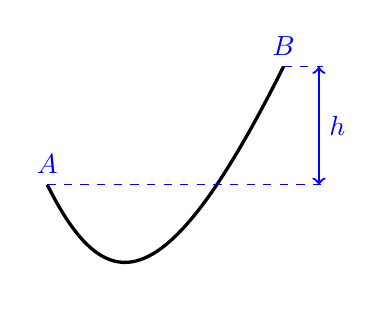
\begin{tikzpicture}
    \draw[very thick] (0,1.5) node[above,blue] {$A$} .. controls
    (0.75,0) and (1.5,0).. (3,3) node[above,blue] {$B$};
    \draw[dashed,blue] (0,1.5) -- (3.5,1.5);
    \draw[dashed,blue] (3,3) -- (3.5,3);
    \draw[blue,thick,<->] (3.45,3) -- (3.45,1.5) node[right,midway] {$h$};
  \end{tikzpicture}
}